% =====================================================================
% PHẦN 9.1: BIỂU DIỄN CẤU TRÚC PHÂN CẤP (DISPLAYING HIERARCHICAL STRUCTURES)
% Người dịch: Nguyễn Khắc Huy (MSSV: 23001525)
% Học liệu: Interactive Data Visualization - Foundations, Techniques, and Applications (2nd Ed.)
% Tác giả: Matthew O. Ward, Georges Grinstein, Daniel Keim
% Phạm vi: Trang in 320–326 (PDF: Trang 342–348)
% =====================================================================

\documentclass[12pt,a4paper,openany]{book}

\usepackage{fontspec}
\usepackage{polyglossia}
\setmainlanguage{vietnamese}

\IfFontExistsTF{Noto Serif}{
  \setmainfont{Noto Serif}[Ligatures=TeX]
  \setsansfont{Noto Sans}
  \setmonofont{Noto Sans Mono}
}{
  \setmainfont{Times New Roman}[Ligatures=TeX]
  \setsansfont{Arial}
  \setmonofont{Consolas}
}

\usepackage[a4paper,top=2.5cm,bottom=2.5cm,left=3cm,right=2cm,headheight=16pt]{geometry}
\usepackage{setspace}
\onehalfspacing

\usepackage{titlesec}
\titleformat{\chapter}[display]
  {\normalfont\huge\bfseries}
  {\chaptertitlename\ \thechapter}
  {20pt}{\Huge}
\titlespacing*{\chapter}{0pt}{0pt}{40pt}

\usepackage{fancyhdr}
\pagestyle{fancy}
\fancyhf{}
\fancyhead[LE,RO]{\thepage}
\fancyhead[RE]{\nouppercase{\leftmark}}
\fancyhead[LO]{\nouppercase{\rightmark}}
\renewcommand{\headrulewidth}{0.4pt}

\usepackage{amsmath}
\usepackage{amssymb}
\usepackage{graphicx}
\usepackage[dvipsnames]{xcolor}
\usepackage{csquotes}
\usepackage{placeins}
\usepackage[hidelinks]{hyperref}

\begin{document}

\chapter*{Phần 9.1. \newline Biểu diễn cấu trúc Phân cấp}
\addcontentsline{toc}{chapter}{Phần 9.1. Biểu diễn cấu trúc Phân cấp}
\markboth{Phần 9.1. Biểu diễn cấu trúc Phân cấp}{}

Cây, hay cấu trúc phân cấp (ta sẽ dùng hai thuật ngữ này thay thế cho nhau), là một trong những cấu trúc phổ biến nhất để lưu giữ thông tin quan hệ. Chính vì vậy, rất nhiều kỹ thuật trực quan hóa đã được phát triển để hiển thị loại thông tin này. Ta có thể chia các kỹ thuật đó thành hai lớp thuật toán: lấp đầy không gian và không lấp đầy không gian. Phần còn lại của mục này sẽ trình bày chi tiết cách cài đặt các thuật toán trực quan hóa loại dữ liệu này.

\section*{9.1.1. Các phương pháp lấp đầy không gian}
\addcontentsline{toc}{section}{Phần 9.1.1. Các phương pháp lấp đầy không gian}

Đúng như tên gọi, các kỹ thuật lấp đầy không gian tận dụng tối đa không gian hiển thị. Điều này đạt được bằng cách dùng phép đặt kề để hàm ý quan hệ, thay vì biểu đạt quan hệ bằng những cạnh nối các đối tượng dữ liệu như ở các cách tiếp cận khác. Hai hướng tiếp cận phổ biến nhất để sinh ra các cấu trúc phân cấp lấp đầy không gian là bố cục chữ nhật và bố cục xuyên tâm.

\subsubsection{Bố cục chữ nhật (Treemap)}

Treemap [206] cùng vô số biến thể của nó là một cách biểu diễn thay thế cho biểu đồ Venn, và là dạng phổ biến nhất của bố cục chữ nhật lấp đầy không gian. Trong treemap cơ bản, một hình chữ nhật được chia đệ quy thành các lát, luân phiên cắt theo phương ngang và phương dọc, dựa trên số lượng phần tử của các cây con ở tầng đang xét. Mã giả của quá trình này được cho ở Hình \ref{fig:treemap_code}, và một ví dụ được trình bày ở Hình \ref{fig:treemap}.

Như đã đề cập, nhiều biến thể của treemap đã được đề xuất và phát triển kể từ khi kỹ thuật này ra đời, trong đó có treemap vuông hóa (squarified treemap) [51] (nhằm giảm bớt sự xuất hiện của những hình chữ nhật dài và mảnh)\footnote{Tỉ lệ khung hình (aspect ratio) của một ô chữ nhật được định nghĩa là $\max(w/h, h/w)$. Thuật toán chia lát cắt luân phiên ban đầu (slice-and-dice) thường tạo ra các ô rất dài và hẹp khi có nhiều node lá (tỉ lệ khung hình lớn), gây khó khăn cho việc tương tác chọn lựa bằng chuột, ước lượng diện tích bằng mắt và hiển thị nhãn văn bản. Squarified treemap tối ưu hóa việc phân chia sao cho tỉ lệ khung hình của mỗi ô xấp xỉ 1 (gần với hình vuông nhất có thể).} và treemap lồng nhau (nested treemap) [206] (nhằm làm nổi bật cấu trúc phân cấp).

\begin{figure}[htbp]
\centering
\par\noindent\rule{0.95\linewidth}{0.5pt}\par\vspace{4pt}
\begin{minipage}{0.9\linewidth}
\singlespacing
\footnotesize
\begin{verbatim}
Start: Main Program
  Width = width of rectangle
  Height = height of rectangle
  Node = root node of the tree
  Origin = position of rectangle, e.g., [0,0]
  Orientation = direction of cuts, alternating
                between horizontal and vertical
  Treemap(Node, Orientation, Origin, Width, Height)
End: Main Program

Treemap(node n, orientation o, position orig, hsize w, vsize h)
  if n is a terminal node (i.e., it has no children)
    draw_rectangle(orig, w, h)
    return
  for each child of n (child_i), get number of terminal nodes in subtree
  sum up number of terminal nodes
  compute percentage of terminal nodes in n from each subtree (percent_i)
  if orientation is horizontal
    for each subtree
      compute offset of origin based on origin and width (offset_i)
      treemap(child_i, vertical, orig + offset_i, w * percent_i, h)
  else
    for each subtree
      compute offset of origin based on origin and height (offset_i)
      treemap(child_i, horizontal, orig + offset_i, w, h * percent_i)
End: Treemap
\end{verbatim}
\end{minipage}
\par\vspace{6pt}\noindent\rule{0.95\linewidth}{0.5pt}\par
\caption{Mã giả vẽ một cấu trúc phân cấp bằng treemap.}
\label{fig:treemap_code}
\end{figure}

\begin{figure}[htbp]
    \centering
    \begin{minipage}{0.48\linewidth}
        \centering
        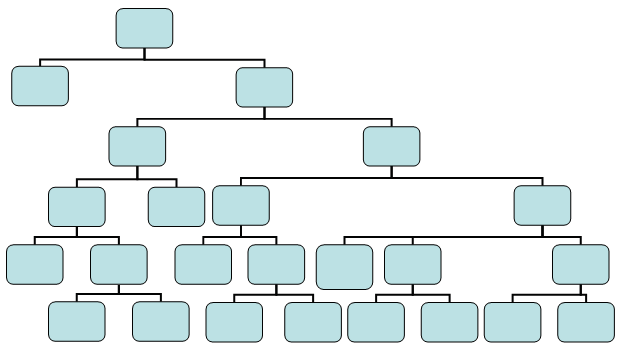
\includegraphics[width=0.85\linewidth]{img/fig9-2a-hierarchy.png}
        \par\vspace{4pt}{\small (a) Cấu trúc phân cấp mẫu}
    \end{minipage}\hfill
    \begin{minipage}{0.48\linewidth}
        \centering
        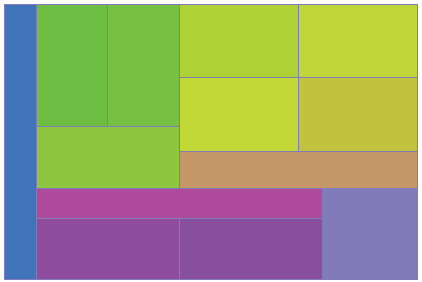
\includegraphics[width=0.85\linewidth]{img/fig9-2b-treemap.png}
        \par\vspace{4pt}{\small (b) Treemap tương ứng}
    \end{minipage}
    \caption{Một cấu trúc phân cấp mẫu và biểu đồ treemap tương ứng.}
    \label{fig:treemap}
\end{figure}

\FloatBarrier
\subsubsection{Bố cục xuyên tâm (Biểu đồ Sunburst)}

Các phương pháp mô tả ở trên được tổ chức bằng những phép chia theo phương ngang và phương dọc để biểu đạt cấu trúc phân cấp. Tuy nhiên, còn nhiều hướng tiếp cận khác cũng khả dĩ, chẳng hạn những hướng chia không gian theo hướng xuyên tâm (radial). Các kỹ thuật trực quan hóa phân cấp lấp đầy không gian theo hướng xuyên tâm, đôi khi được gọi là biểu đồ sunburst [393], đặt node gốc của cấu trúc phân cấp ở tâm màn hình và dùng các vành tròn lồng nhau để biểu đạt các tầng của cấu trúc\footnote{Biểu đồ sunburst về bản chất là một dạng tương đương trong hệ tọa độ cực (polar coordinates) của treemap, trong đó góc quét đại diện cho độ rộng phân vùng và bán kính thể hiện độ sâu phân cấp. Điểm vượt trội của sunburst là người xem dễ dàng nhận biết cấu trúc phân nhánh và quan hệ phả hệ hơn treemap phẳng, tuy nhiên diện tích hiển thị của các node lá ở tầng sâu bên ngoài bị kéo dãn nhanh chóng do chu vi vành tròn tăng theo bán kính.}. Mỗi vành được chia dựa trên số node ở tầng tương ứng. Các kỹ thuật này đi theo một chiến lược tương tự treemap, ở chỗ số node lá trong một cây con sẽ quyết định lượng không gian màn hình được cấp phát cho cây con đó. Tuy nhiên, khác với treemap vốn dành phần lớn không gian màn hình để thể hiện các node lá, các kỹ thuật xuyên tâm còn thể hiện cả những node trung gian. Quá trình này được mô tả bằng mã giả ở Hình \ref{fig:sunburst_code}, và một ví dụ được trình bày ở Hình \ref{fig:sunburst}.

Với những kỹ thuật lấp đầy không gian này cũng như các kỹ thuật khác, màu sắc có thể được dùng để biểu đạt nhiều thuộc tính, chẳng hạn một giá trị gắn với node (ví dụ: phân loại), hoặc để củng cố các quan hệ phân cấp --- chẳng hạn các node anh em và node cha có thể mang màu sắc tương đồng, như thấy ở Hình \ref{fig:sunburst}. Các ký hiệu và dấu hiệu khác cũng có thể được nhúng vào các phân đoạn hình chữ nhật hoặc hình tròn để truyền đạt những đặc trưng dữ liệu khác.

\begin{figure}[htbp]
\centering
\par\noindent\rule{0.95\linewidth}{0.5pt}\par\vspace{4pt}
\begin{minipage}{0.9\linewidth}
\singlespacing
\footnotesize
\begin{verbatim}
Start: Main Program
  Start = start angle for a node (initially 0)
  End = end angle for a node (initially 360)
  Origin = position of center of sunburst, e.g., [0,0]
  Level = current level of hierarchy (initially 0)
  Width = thickness of each radial band - based on
          max depth and display size
  Sunburst(Node, Start, End, Level)
End: Main Program

Sunburst(node n, angle st, angle en, level l)
  if n is a terminal node (i.e., it has no children)
    draw_radial_section(Origin, st, en, l * Width, (l+1) * Width)
    return
  for each child of n (child_i), get number of terminal nodes in subtree
  sum up number of terminal nodes
  compute percentage of terminal nodes in n from each subtree (percent_i)
  for each subtree
    compute start/end angle based on size of subtrees,
            order, and angle range
    Sunburst(child_i, st_i, en_i, l+1)
End: Sunburst
\end{verbatim}
\end{minipage}
\par\vspace{6pt}\noindent\rule{0.95\linewidth}{0.5pt}\par
\caption{Mã giả vẽ một cấu trúc phân cấp bằng biểu đồ sunburst.}
\label{fig:sunburst_code}
\end{figure}

\begin{figure}[htbp]
    \centering
    \begin{minipage}{0.48\linewidth}
        \centering
        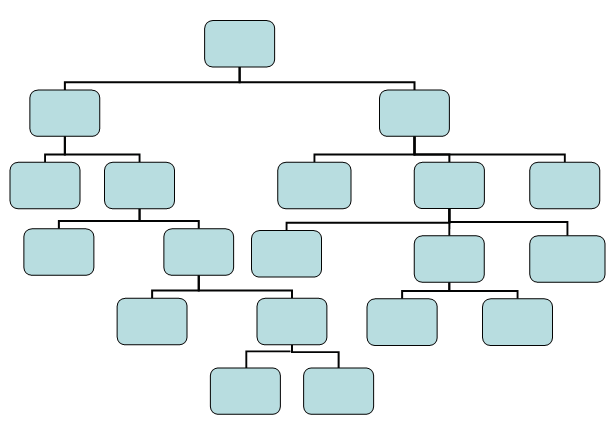
\includegraphics[width=0.85\linewidth]{img/fig9-4a-hierarchy.png}
        \par\vspace{4pt}{\small (a) Cấu trúc phân cấp mẫu}
    \end{minipage}\hfill
    \begin{minipage}{0.48\linewidth}
        \centering
        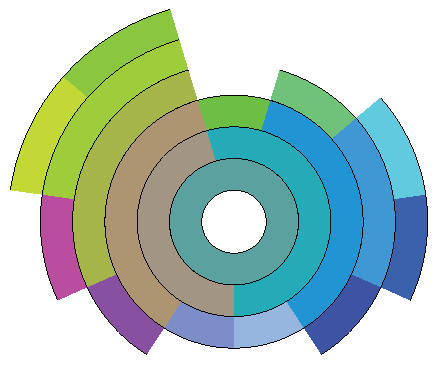
\includegraphics[width=0.85\linewidth]{img/fig9-4b-sunburst.png}
        \par\vspace{4pt}{\small (b) Biểu đồ sunburst tương ứng}
    \end{minipage}
    \caption{Một cấu trúc phân cấp mẫu và biểu đồ sunburst tương ứng.}
    \label{fig:sunburst}
\end{figure}

\FloatBarrier
\section*{9.1.2. Các phương pháp không lấp đầy không gian}
\addcontentsline{toc}{section}{Phần 9.1.2. Các phương pháp không lấp đầy không gian}

\subsubsection{Sơ đồ node-link cho cấu trúc cây}

Cách biểu diễn phổ biến nhất dùng để trực quan hóa quan hệ cây hay quan hệ phân cấp là sơ đồ node-link. Sơ đồ tổ chức, cây gia phả và bảng ghép cặp thi đấu chỉ là một vài trong số những ứng dụng thường gặp của loại sơ đồ này. Việc vẽ những cây như vậy chịu ảnh hưởng nhiều nhất bởi hai yếu tố: bậc phân nhánh (fan-out degree, ví dụ: số node anh em mà một node cha có thể có) và độ sâu (depth, ví dụ: node nằm xa node gốc nhất). Những cây bị ràng buộc chặt ở một hoặc cả hai khía cạnh này --- chẳng hạn cây nhị phân, hay cây chỉ có ba đến bốn tầng --- thường dễ vẽ hơn nhiều so với những cây ít bị ràng buộc hơn.

Khi thiết kế thuật toán vẽ bất kỳ sơ đồ node-link nào (không riêng gì cây), ta phải cân nhắc ba nhóm nguyên tắc thường mâu thuẫn với nhau: quy ước vẽ, ràng buộc và tính thẩm mỹ. Các quy ước có thể bao gồm việc giới hạn cạnh chỉ được là một đoạn thẳng đơn, một chuỗi các đoạn thẳng vuông góc, các đường gấp khúc đa giác, hoặc các đường cong. Những quy ước khác có thể là đặt các node trên một lưới cố định, hoặc buộc mọi node anh em phải có cùng vị trí theo phương dọc. Các ràng buộc có thể bao gồm yêu cầu một node cụ thể phải nằm ở tâm màn hình, hoặc một nhóm node phải được đặt gần nhau, hoặc một số liên kết nhất định bắt buộc phải đi từ trên xuống dưới hoặc từ trái sang phải. Mỗi nguyên tắc nêu trên đều có thể được dùng để dẫn dắt việc thiết kế thuật toán.

Tuy nhiên, tính thẩm mỹ thường có tác động đáng kể đến khả năng diễn giải của một hình vẽ cây hay đồ thị, song lại thường dẫn đến những nguyên tắc xung đột nhau\footnote{Trong lĩnh vực vẽ đồ thị (Graph Drawing), việc tối ưu hóa đồng thời các tiêu chí thẩm mỹ (đặc biệt là cực tiểu hóa số giao cắt cạnh --- crossing minimization) trên đồ thị tổng quát là bài toán thuộc lớp NP-khó (NP-hard). Tuy nhiên, đối với cấu trúc cây phân cấp, các thuật toán kinh điển như Reingold--Tilford (1981) hay Walker (1990) có thể đạt được tính thẩm mỹ cao và đối xứng với độ phức tạp thời gian tuyến tính $O(|V|)$ và không có cạnh nào bị cắt nhau.}. Một số quy tắc thẩm mỹ điển hình bao gồm:

\begin{itemize}
    \item giảm thiểu số giao cắt đường,
    \item duy trì một tỉ lệ khung hình dễ nhìn,
    \item giảm thiểu tổng diện tích của hình vẽ,
    \item giảm thiểu tổng độ dài các cạnh,
    \item giảm thiểu số điểm gấp khúc trên các cạnh,
    \item giảm thiểu số lượng góc hoặc độ cong khác nhau được sử dụng,
    \item hướng tới một cấu trúc đối xứng.
\end{itemize}

Đối với cây, đặc biệt là cây cân bằng, việc thiết kế thuật toán tuân thủ nhiều --- nếu không muốn nói là hầu hết --- các nguyên tắc trên là tương đối dễ dàng. Chẳng hạn, một thủ tục vẽ cây đơn giản được trình bày dưới đây (kết quả mẫu được thể hiện ở Hình \ref{fig:nodelink}):

\begin{enumerate}
    \item Cắt vùng vẽ thành các dải có chiều cao bằng nhau, dựa trên độ sâu của cây.
    \item Với mỗi tầng của cây, xác định cần vẽ bao nhiêu node.
    \item Chia mỗi dải thành các hình chữ nhật có kích thước bằng nhau, dựa trên số node ở tầng đó.
    \item Vẽ mỗi node vào tâm hình chữ nhật tương ứng của nó.
    \item Vẽ một liên kết từ điểm giữa cạnh dưới của mỗi node đến điểm giữa cạnh trên của (các) node con của nó.
\end{enumerate}

\begin{figure}[htbp]
    \centering
    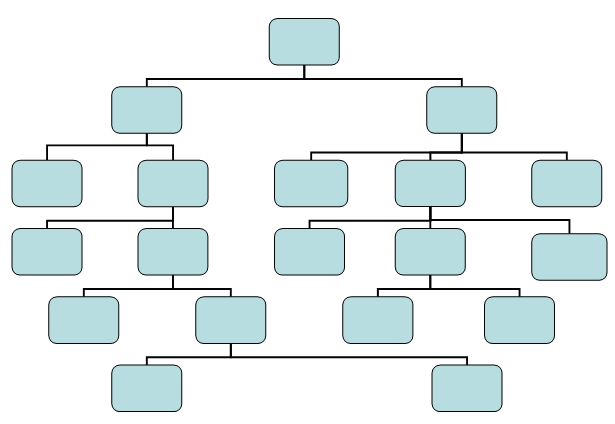
\includegraphics[width=0.65\linewidth]{img/fig9-5-node-link.png}
    \caption{Một ví dụ trực quan hóa cấu trúc phân cấp bằng sơ đồ node-link đơn giản, sử dụng khoảng cách đều nhau ở mỗi tầng.}
    \label{fig:nodelink}
\end{figure}

Có thể thực hiện nhiều cải tiến cho thuật toán khá cơ bản này nhằm nâng cao hiệu quả sử dụng không gian và đưa các node con lại gần node cha hơn. Một số cải tiến đó gồm:

\begin{itemize}
    \item Thay vì dùng khoảng cách đều và căn giữa, hãy chia mỗi tầng dựa trên số node lá thuộc về mỗi cây con.
    \item Trải đều các node lá trên toàn vùng vẽ và căn các node cha vào chính giữa, phía trên chúng.
    \item Thêm một khoảng đệm giữa các node liền kề không phải anh em để làm nổi bật quan hệ.
    \item Nếu có thể, sắp xếp lại thứ tự các cây con của một node để đạt được độ đối xứng và cân đối cao hơn.
    \item Đặt node gốc ở tâm màn hình và bố trí các node con theo hướng xuyên tâm, thay vì theo phương dọc.
\end{itemize}

\FloatBarrier
\subsubsection{Hiển thị trong không gian ba chiều (Cone Tree)}

Đối với những cây lớn, một hướng tiếp cận phổ biến là sử dụng chiều thứ ba, bổ sung thêm các công cụ xoay, tịnh tiến và thu phóng. Kỹ thuật nổi tiếng nhất trong số đó được gọi là \textit{cone tree} (cây hình nón) [341]\footnote{Cone tree được phát minh tại trung tâm nghiên cứu Xerox PARC (Robertson et al., 1991). Mặc dù là một bước đột phá trong trực quan hóa tương tác 3D lúc bấy giờ, trong thực tiễn người ta vẫn ưa chuộng các cấu trúc cây 2D tương tác dạng thu gọn/mở rộng (collapsible/zoomable trees) hơn, bởi vì không gian 3D làm tăng gánh nặng nhận thức không gian (spatial cognitive load) và dễ gặp hiện tượng các nhánh phía trước che khuất (occlusion) các node quan trọng phía sau.}. Trong bố cục này, các node con của một node được sắp xếp theo hướng xuyên tâm tại những góc cách đều nhau, rồi được dịch chuyển theo phương vuông góc với mặt phẳng. Hai tham số then chốt của quá trình này là bán kính và khoảng dịch chuyển; thay đổi chúng sẽ ảnh hưởng đến mật độ của hình hiển thị và mức độ che khuất. Ở mức tối thiểu, chúng phải được đặt sao cho các nhánh riêng biệt của cây không rơi vào cùng một vùng của không gian ba chiều. Một cách để bảo đảm điều này là cho bán kính tỉ lệ nghịch với độ sâu của node trong cây. Theo cách đó, những node gần node gốc sẽ được tách xa nhau đáng kể, còn những node ở gần đáy cây thì nằm sát nhau hơn. Một ví dụ được thể hiện ở Hình \ref{fig:conetree}.

\begin{figure}[htbp]
    \centering
    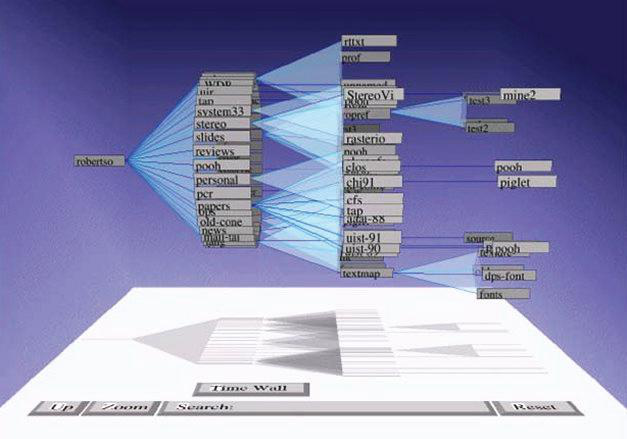
\includegraphics[width=0.75\linewidth]{img/fig9-6-cone-tree.png}
    \caption{Một ví dụ về cấu trúc phân cấp được hiển thị bằng cone tree [341]. (Hình ảnh \copyright~1991 Association of Computing Machinery. In lại với sự cho phép, do PARC, Inc. cung cấp.)}
    \label{fig:conetree}
\end{figure}

\FloatBarrier
\clearpage
% ---------------------------------------------------------------------
% BẢNG ĐỐI CHIẾU THUẬT NGỮ CHUYÊN NGÀNH
% ---------------------------------------------------------------------
\section*{Bảng đối chiếu thuật ngữ chuyên ngành}
\addcontentsline{toc}{section}{Bảng đối chiếu thuật ngữ chuyên ngành}

\begin{table}[htbp]
\centering
\small
\begin{tabular}{|p{6.5cm}|p{7.5cm}|}
\hline
\textbf{Thuật ngữ tiếng Anh gốc} & \textbf{Bản dịch tiếng Việt} \\
\hline
hierarchy / hierarchical structure & cấu trúc phân cấp \\
tree & cây \\
node & node \\
edge & cạnh \\
link & liên kết \\
root node & node gốc \\
child node & node con \\
parent node & node cha \\
sibling node & node anh em \\
terminal node & node lá \\
intermediate node & node trung gian \\
subtree & cây con \\
depth & độ sâu \\
level & tầng \\
space-filling & lấp đầy không gian \\
non--space-filling & không lấp đầy không gian \\
display space & không gian hiển thị \\
juxtapositioning & phép đặt kề \\
treemap & treemap \\
squarified treemap & treemap vuông hóa \\
nested treemap & treemap lồng nhau \\
sunburst display & biểu đồ sunburst \\
Venn diagram & biểu đồ Venn \\
radial layout & bố cục xuyên tâm \\
node-link diagram & sơ đồ node-link \\
fan-out degree & bậc phân nhánh \\
cone tree & cone tree (cây hình nón) \\
drawing conventions & quy ước vẽ \\
constraints & ràng buộc \\
aesthetics & tính thẩm mỹ \\
line crossings & giao cắt đường \\
aspect ratio & tỉ lệ khung hình \\
bends in the edges & điểm gấp khúc trên cạnh \\
occlusion & sự che khuất \\
pseudocode & mã giả \\
binary tree & cây nhị phân \\
balanced tree & cây cân bằng \\
\hline
\end{tabular}
\caption{Bảng đối chiếu thuật ngữ chuyên ngành trong phần 9.1.}
\label{tab:glossary_9_1}
\end{table}

\end{document}
